\subsection{Classifying attacks}
Attacks are often classified along two axes falling into one of four categories: \cite{FX2010}.

\begin{itemize}
  \item \textbf{Hardware tampering}
    \begin{itemize}
      \item[1.] Invasive - Attacks which try to read the actual data either by intercepting or directly reading data. An example of this could be to connect a wire onto the data bus and view the data transfers or doing some sort of memory inspection.
      \item[2.] Non-invasive - Attacks which do not read the actual data, but exploits externally available information. External information can be observations on running time, power consumption and such.
    \end{itemize}
  \item \textbf{System tampering}
    \begin{itemize}
      \item[3.] Active - Attacks that tries to change the behaviour of some function on the device, such as introducing a fault in the computation to cause a leak of information, or cold-booting the device to perform memory dumps \cite{Halderman2008LestKeys}.
      \item[4.] Passive - Attacks that only observes a devices behaviour, without affecting it. No signs of compromise or failure.
    \end{itemize}
\end{itemize}

Figure \ref{fig:sca_classification} visualizes these classifications with hardware tampering along the x axis and system tampering along the y axis.
The safety that Hermes intends to provide is against timing attacks and information leakage which includes cold boot attacks.
Timing attacks are non-invasive and passive as the attacker only observes the running time of the process.
Cold boot attacks are active attacks as they perform memory dumps, but can be either invasive or non-invasive exemplified in \cite{Halderman2008LestKeys} where, in one attack, researchers freeze the chip thereby tampering with the hardware.

\begin{figure}[htp]
  \resizebox{0.9\columnwidth}{!}{%
      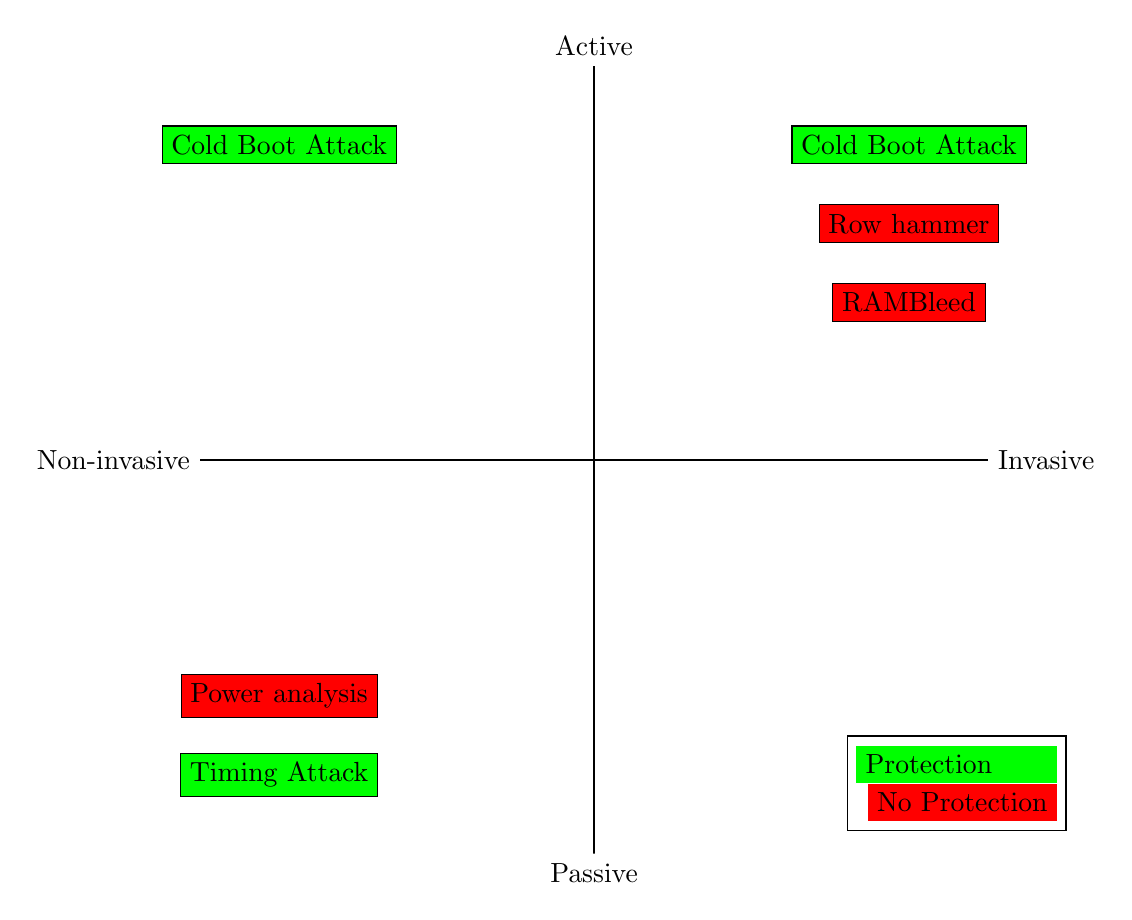
\begin{tikzpicture}
        \draw [thick] (0,5) node (yaxis) [above] {Active}
          |- (0,-5) node (yaxis) [below] {Passive}
          |- (5,0) node (xaxis) [right] {Invasive}
          |- (-5,0) node (xaxis) [left] {Non-invasive};
        \node[draw, fill=green] at (-4,4) {Cold Boot Attack};
        \node[draw, fill=green] at (4,4) {Cold Boot Attack};
        \node[draw, fill=red] at (-4,-3) {Power analysis};
        \node[draw, fill=green] at (-4,-4) {Timing Attack};
        \node[draw, fill=red] at (4,3) {Row hammer};
        \node[draw, fill=red] at (4,2) {RAMBleed};
        % Legend
        \matrix [draw, below left] at (6,-3.5) {
          \node [fill=green] {Protection\ \ \ \ \ \ \ }; \\
          \node [fill=red] {No Protection}; \\
        }; 
      \end{tikzpicture}%
  }
  \caption{Some side-channel attacks and their classifications} 
  \label{fig:sca_classification}
\end{figure}

Side-channels attacks have been gaining a lot of attention recently by device manufactorers. Especially the non-invasive, passive attacks which are hard to spot and can generally be performed using relatively cheap equipment.
